\documentclass[tikz,border=3pt]{standalone}
\usepackage[utf8]{inputenc}
\usepackage[T1]{fontenc}
\usepackage{lmodern}
\renewcommand{\familydefault}{\sfdefault}
\usepackage{sansmath}\sansmath
\usepackage{chemfig}
\usepackage{pgfplots}\pgfplotsset{compat=1.18,/pgf/number format/use comma,/pgf/number format/1000 sep={.}}
\usetikzlibrary{arrows.meta,calc,positioning,decorations.pathmorphing,decorations.pathreplacing,patterns}
% paleta del sitio
\definecolor{nar}{HTML}{E8680C}\definecolor{narc}{HTML}{FFB35C}\definecolor{hielo}{HTML}{FFF3E8}
\definecolor{tinta}{HTML}{1D1D1F}\definecolor{gris}{HTML}{6E6E73}\definecolor{lila}{HTML}{7C5CF0}
\definecolor{azul}{HTML}{2F6FD6}\definecolor{menta}{HTML}{17A673}\definecolor{coral}{HTML}{E8342A}
\begin{document}
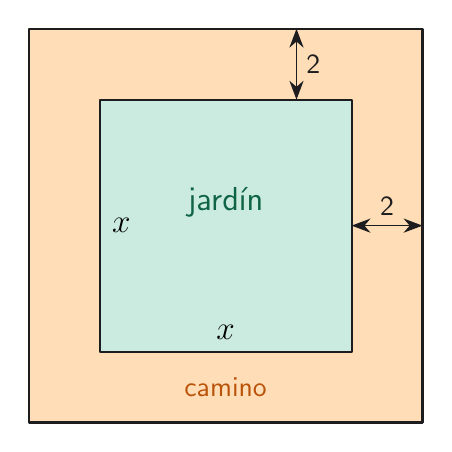
\begin{tikzpicture}[font=\large,line join=round,>={Stealth[length=2.4mm]}]
\def\s{3.2}\def\c{0.9}
\draw[tinta,thick,fill=narc!45] (0,0) rectangle (\s+2*\c,\s+2*\c);
\draw[tinta,thick,fill=menta!22] (\c,\c) rectangle (\c+\s,\c+\s);
\node[text=menta!60!black] at (\c+\s/2,\c+\s/2+0.3) {jardín};
\node[text=nar!80!black,font=\normalsize] at (\c+\s/2,\c/2) {camino};
\node[above=1pt] at (\c+\s/2,\c) {$x$};
\node[right=1pt] at (\c,\c+\s/2) {$x$};
\draw[tinta,<->] (\c+\s,\c+\s/2) -- (2*\c+\s,\c+\s/2) node[midway,above,font=\normalsize] {2};
\draw[tinta,<->] (\c+\s/2+0.9,\c+\s) -- (\c+\s/2+0.9,2*\c+\s) node[midway,right,font=\normalsize] {2};
\end{tikzpicture}
\end{document}
